\documentclass[11pt]{article}

\usepackage[margin = 1in]{geometry}
\usepackage{mathtools}
\usepackage{float}
\usepackage{graphicx}

\usepackage{hyperref}

\usepackage[backend = biber, style = phys, sorting = ynt]{biblatex}
\addbibresource{citations.bib}

\title{SuperconGAN: A Library to Generate and Predict Superconductive Materials}

\author{
    Rajeev Atla\\
    \texttt{\href{mailto:rajeev@rajeevatla.com}{rajeev@rajeevatla.com}}
}

\date{}

\begin{document}

\maketitle

\begin{abstract}
TODO
\end{abstract}

\section{Introduction}

Achieving a room-temperature superconductor is considered the hallmark of condensed matter physics.
However, researchers have faced many challenges in their search for such a material, including long, costly production times and sensitivity toward environmental conditions \cite{blank1988} \cite{zaki_saleem_anwar_2013}.
Although the advent of novel superconductors such as Van der Waals heterostructures, including twisted bilayer graphene (TBG) \cite{tbg_2018}, has lessened this, searching through the entire phase diagrams of even these materials would likely take decades without a way to accelerate the process of discovery.
One possible way to solve this problem is to use a data-based method, using previous, already discovered superconductors to make inferences about potential ones.
It would be of great assistance to researchers in the field to be able to differentiate between non-superconductors and superconductors through a data-based method utilizing already known superconductors.
Recent work \cite{hamidieh2018} has used easily observable characteristics to predict critical temperature.
However, no clear association has been found yet between the easily observable characteristics of a material and its superconductive phase diagram, so a supervised learning approach isn't realizable.
Herein, we attempt a solution to this problem: an unsupervised generative adversarial network (GAN) that allows researchers to evaluate materials to further investigate for possible supercondctivity.
Further, this GAN only uses easily observable characteristics such as valence, atomic radius, etc., allowing researchers to determine whether a material can exhibit supercondctivity. 
Such a method would also be able to generate possible superconductive materials to be tested, further pushing the pace of existing research by perpetually pointing researchers towards potentially new directions.

\section{Methods}

To obtain the data, we use the Supercon database \cite{hamidieh2018}, obtained from the UCI machine learning repository \cite{UCI}.
The dataset contains 81 features extracted from 21263 superconductors, along with their chemical formulae and critical temperatures.
In order to generate and evaluate superconductive materials, we remove the critical temperatures from consideration, keeping only easily physical characteristics such as thermal conductivity, atomic radius, electron affinity, and atomic mass.

We then train a GAN upon this cleaned dataset. Specifically, we use the Conditional Tabular GAN (CTGAN) library \cite{CTGAN} to generate this data, for its ability to also generate conditional data.
SuperconGAN then functions as a wrapper around CTGAN, allowing researchers to easily synthesize data without delving deeply into CTGAN's syntax.

A GAN works \cite{GAN} by generating data from a random noise vector. One of the two GAN components, the generator, creates a map between this random noise vector and a set of fake data.
The other GAN component, the discriminator, tries to tell the difference between this fake data and the real data, and sends feedback to the generator.
This generator uses this feedback to update its mapping to try and fool the discriminator.
This process results in the production of data that closely mimics the real data.

To evaluate the quality of the data produced independently of the GAN, we use the single table evaluation function provided by the Synthetic Data Vault (SDV) \cite{patki_wedge_veeramachaneni_2016}: SDMetrics.
This function compares the results of several machine learning models (see \ref{appendix:Metrics}) between the synthetic and real data.

To allow researchers to evaluate the GAN's training before it finishes, SuperconGAN allows the display of generator and discriminator losses.
The discriminator loss is defined as the difference between the fake data and the real data.
The generator loss is the difference between the cross entropy between the two datasets and the mean of the fake data.

\section{Results}
We present the generator and discriminator losses in Figure 1.

\newpage

\begin{figure}[H]
    \caption{The generator and discriminator losses plotted together, after being averaged across $n=3$ trials. Due to the nature of the noise vector used to train the generator, the losses also reflect this noise.}
    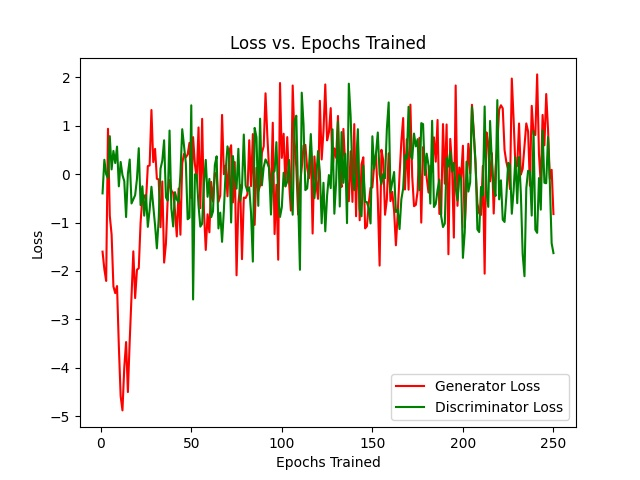
\includegraphics{graph1}
    \centering
\end{figure}

\newpage

\begin{figure}[H]
    \caption{The generator and discriminator losses are averaged across $n=3$ trials and a 95\% confidence interval is constructed at each epoch.
            Note: same data as Figure 1.}
    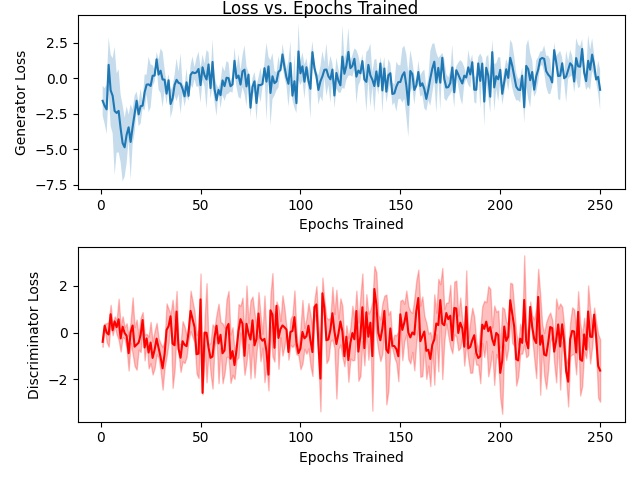
\includegraphics{graph2}
    \centering
\end{figure}

\newpage

We present the results of the evaluation function, as a function of the number of epochs the GAN is trained, in Figure 3.

\begin{figure}[H]
    \caption{The evaluation function is significantly less noisy than the losses plotted. Note the diminishing marginal returns exhibited.}
    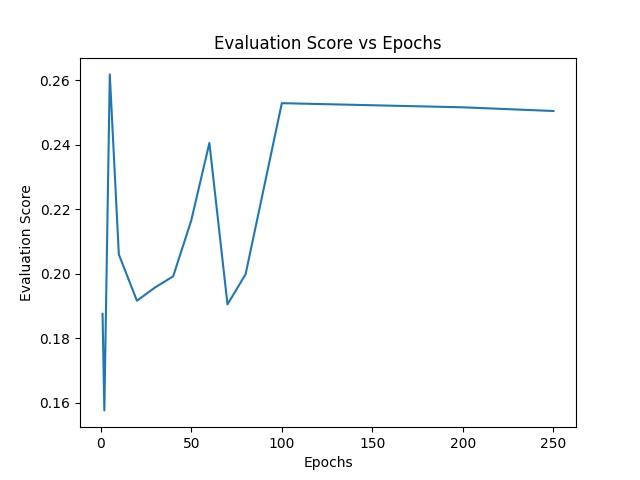
\includegraphics{graph3}
    \centering
\end{figure}

\newpage

\section{Conclusion}
In this work, we discuss a novel GAN-based approach towards the study of superconductor data.
This approach would allow researchers to utilize existing data-based approaches more effectively, as one of the largest bottlenecks to a machine learning problem is the availability of data.
Existing methods of calculating the critical temperature of a superconductor could be augmented by the data created by SuperconGAN, allowing more accurate estimates.
Further work could also map the parameter space, allowing researchers to see what physical characteristics are really necessary to exhibit superconductivity.
Another possible research direction could be differentiating between type I and type II superconductors, and further exploring the physical characteristics of each.

This work could also be combined with existing deep learning models \cite{https://doi.org/10.1002/adma.202000953} that utilize the phase space to make predictions, amplifying their ability by also supplying data about the physical characteristics of a material.

\newpage

\section{Acknowledgements}
I would like to thank Leo Lo and Dr. Serena McCalla for all their support through iResearch Institute 2020.

\section{References}

\printbibliography[heading = none]

\appendix
\section{Appendix: Evaluation Metrics}
\label{appendix:Metrics}
We use the evaluate function of SDMetrics \cite{patki_wedge_veeramachaneni_2016}, which uses these metrics to evaluate the quality of the data produced.

\begin{table}[h]
    \caption{\textbf{Error Metrics}}
    \begin{center}
        \begin{tabular}{ c c }
            \textbf{Metric} & \textbf{Return Value} \\
            Bayesian Network Likelihood & Average likelihood of of synthetic data using Bayesian Network \\
            Bayesian Network Log Likelihood & Average log likelihood of of synthetic data using Bayesian Network \\
            Gaussian Mixture Log Likelihood & Average log likelihood of of synthetic data using Gaussian Mixture \\
            Logistic Detection & One minus average ROC AUC score from logistic regression \\
            SVC Detection & One minus average ROC AUC score from support vector classification \\
            CS Test & Chi-squared test test statistic \\
            KS Test & Kolmogorov-Smirnov test statistic \\
            Continouus KL Divergence & Kullback-Leibler divergence \\
        \end{tabular}
    \end{center}
\end{table}
Further, SDmetrics takes the metrics whose values don't lie on $[-1, 1]$ and normalizes them using a hyperbolic tangent. The average of the normalized metric is returned.

\end{document}
